\documentclass[12pt, a4paper, oneside]{Thesis} % Paper size, default font size and one-sided paper
\usepackage{wrapfig}
\usepackage{lscape}
\usepackage{rotating}
\usepackage{graphicx}
\usepackage{caption}
\usepackage{amsmath}
\usepackage{gensymb}

\usepackage{lineno,hyperref}
\modulolinenumbers[5]


\usepackage{amssymb}
\usepackage{graphicx}
\usepackage{array}
\usepackage{float}
\usepackage{placeins}
\usepackage{stackengine}
\usepackage{url}
\usepackage{numprint}
\usepackage{caption}

\usepackage{booktabs}  
\usepackage{siunitx}
%\usepackage[showframe=false]{geometry}
\usepackage{subfigure}

\nprounddigits{3}
\newcolumntype{P}[1]{>{\centering\arraybackslash}p{#1}}
\newcolumntype{M}[1]{>{\centering\arraybackslash}m{#1}}

\setstackEOL{\#}
\setstackgap{L}{12pt}


%\usepackage{subcaption} %incompatible with subfig
\graphicspath{{Pictures/}} % Specifies the directory where pictures are stored
\usepackage[sort, numbers]{natbib} % Use the natbib reference package - read up on this to edit the reference style; if you want text (e.g. Smith et al., 2012) for the in-text references (instead of numbers), remove 'numbers' v

\hypersetup{urlcolor=black, colorlinks=false} % Colors hyperlinks in blue - change to black if annoyingv`	

\thesistitle{Detection of Forest Area in SAR images}
\supervisor{Dr. Jayanta Mukhopadhyay}
\degree{Master of Technology}
\degreemajor{Computer Science and Engineering}
\authors{Jeffrey Jose}
\rollno{17CS60R77}
\university{Indian Institute of Technology Kharagpur}
\department{Department of Computer Science and Engineering}
\unisite{http://www.iitkgp.ac.in}
\depsite{http://www.cse.iitkgp.ac.in}
\placeshrt{Kharagpur}
\placelng{Kharagpur - 721302, India}
\datesub{November 14, 2018}
\datesig{November 14, 2018}
\semsub{Autumn Semester, 2018-19}
\keywords{Forest classification, SAR polarimetry,Support vector machine }
\coursecd{Thesis Part-I (CS67101) }

\title{\ttitle} % Defines the thesis title - don't touch this
\begin{document}
%\makeatletter
%\renewcommand*{\NAT@nmfmt}[1]{\textsc{#1}}
%\makeatother

% prints author names as small caps


\frontmatter % Use roman page numbering style (i, ii, iii, iv...) for the pre-content pages

\setstretch{1.6} % Line spacing of 1.6 (double line spacing)

% Define the page headers using the FancyHdr package and set up for one-sided printing
\fancyhead{} % Clears all page headers and footers
\rhead{\thepage} % Sets the right side header to show the page number
\lhead{} % Clears the left side page header

%\pagestyle{fancy} % Finally, use the "fancy" page style to implement the FancyHdr headers

\newcommand{\HRule}{\rule{\linewidth}{0.5mm}} % New command to make the lines in the title page

% PDF meta-data
\hypersetup{pdftitle={\ttitle}}
\hypersetup{pdfsubject=\subjectname}
\hypersetup{pdfauthor=\authornames}
\hypersetup{pdfkeywords=\keywordnames}

%----------------------------------------------------------------------------------------
%	TITLE PAGE
%----------------------------------------------------------------------------------------
\maketitle
%\titlepg % Add a gap in the Contents, for aesthetics

\clearpage % Start a new page

%----------------------------------------------------------------------------------------
%	DECLARATION PAGE
%	Your institution may give you a different text to place here
%----------------------------------------------------------------------------------------


\Declaration% Add a gap in the Contents, for aesthetics


%----------------------------------------------------------------------------------------
%	CERTIFICATE PAGE
%----------------------------------------------------------------------------------------

\addtotoc{Certificate} % Add the "Abstract" page entry to the Contents

\certificate{\addtocontents{toc}{} % Add a gap in the Contents, for aesthetics

\clearpage % Start a new page

%----------------------------------------------------------------------------------------
%	ABSTRACT PAGE
%----------------------------------------------------------------------------------------

\addtotoc{Abstract} % Add the "Abstract" page entry to the Contents

\abstract{\addtocontents{toc}{} % Add a gap in the Contents, for aesthetics

The technology of remote sensing has seen various advancements which aid the accessibility of land surface data. Using this image data, forest regions can be properly mapped and monitored. We propose to detect forest region with the help of active hybrid polarized SAR data. Using the features of the hybrid polarized SAR data such as stokes parameters , m-$\delta$ and a set of reference forest pixels, we try to classify unknown areas, using machine learning models such as maximum likelihood classifier and one-class SVM, as either forest or non-forest.   
}

\clearpage % Start a new page

%----------------------------------------------------------------------------------------
%	LIST OF CONTENTS/FIGURES/TABLES PAGES
%----------------------------------------------------------------------------------------

\pagestyle{fancy} % The page style headers have been "empty" all this time, now use the "fancy" headers as defined before to bring them back

\lhead{\emph{Contents}} % Set the left side page header to "Contents"
\tableofcontents % Write out the Table of Contents

\lhead{\emph{List of Figures}} % Set the left side page header to "List of Figures"
\listoffigures % Write out the List of Figures

\lhead{\emph{List of Tables}} % Set the left side page header to "List of Tables"
\listoftables % Write out the List of Tables

%----------------------------------------------------------------------------------------
%	ABBREVIATIONS
%----------------------------------------------------------------------------------------

\clearpage % Start a new page

\setstretch{1.5} % Set the line spacing to 1.5, this makes the following tables easier to read

\lhead{\emph{Abbreviations}} % Set the left side page header to "Abbreviations"
\listofsymbols{ll} % Include a list of Abbreviations (a table of two columns)
{
\textbf{SAR} & \textbf{S}ynthetic \textbf{A}perture \textbf{R}adar \\
\textbf{GIS} & \textbf{G}eographic \textbf{I}nformation \textbf{S}ystem \\
\textbf{SVM} & \textbf{S}upport \textbf{V}ector \textbf{M}achine \\
%\textbf{Acronym} & \textbf{W}hat (it) \textbf{S}tands \textbf{F}or \\
}

%----------------------------------------------------------------------------------------
%	PHYSICAL CONSTANTS/OTHER DEFINITIONS
%----------------------------------------------------------------------------------------
%
%\clearpage % Start a new page
%
%\lhead{\emph{Physical Constants}} % Set the left side page header to "Physical Constants"
%
%\listofconstants{lrcl} % Include a list of Physical Constants (a four column table)
%{
%Speed of Light & $c$ & $=$ & $2.997\ 924\ 58\times10^{8}\ \mbox{ms}^{-\mbox{s}}$ (exact)\\
%% Constant Name & Symbol & = & Constant Value (with units) \\
%}

%----------------------------------------------------------------------------------------
%	SYMBOLS
%----------------------------------------------------------------------------------------

\clearpage % Start a new page

\lhead{\emph{Symbols}} % Set the left side page header to "Symbols"

\listofnomenclature{lll} % Include a list of Symbols (a two column table)
{
$D^{el}$ & elasticity tensor \\
$\sigma$ & stress tensor \\
$ \varepsilon $ & strain tensor \\
% Symbol & Name & Unit \\

}

%----------------------------------------------------------------------------------------
%	DEDICATION
%----------------------------------------------------------------------------------------
%
%\setstretch{1.3} % Return the line spacing back to 1.3
%
%\pagestyle{empty} % Page style needs to be empty for this page
%
%\dedicatory{For/Dedicated to/To my\ldots} % Dedication text
%
%\addtocontents{toc}{\vspace{2em}} % Add a gap in the Contents, for aesthetics

%----------------------------------------------------------------------------------------
%	THESIS CONTENT - CHAPTERS
%----------------------------------------------------------------------------------------

\mainmatter % Begin numeric (1,2,3...) page numbering

\pagestyle{fancy} % Return the page headers back to the "fancy" style

% Include the chapters of the thesis as separate files from the Chapters folder
% Uncomment the lines as you write the chapters

% Chapter Template

\chapter{Sample} % Main chapter title

\label{Chapter 1} % Change X to a consecutive number; for referencing this chapter elsewhere, use \ref{ChapterX}

\lhead{Chapter 1. \emph{Sample}} % Change X to a consecutive number; this is for the header on each page - perhaps a shortened title

%----------------------------------------------------------------------------------------
%	SECTION 1
%---------------------------------------------------------------------------------------
\section{Introduction}



Give a brief of the chapter and introduce what you will talk about. 


\paragraph{Literature Survey}

This is a sample. Write about referred papers. Cite like this \citep{nip2010cyclic}. Another example would be this \citep{nip2010extremely}. More citations like this \citep{bird2004evaluating}, \citep {tremblay2003seismic} and \citep {alhamaydeh2016key}.

\paragraph{Research gaps}
Typically include research gaps for your study. 
\paragraph{Objective}
Similarly objectives of study. 
\paragraph{Scope}
Define scope of study. 
\paragraph{An algorithm}
How you could refer to figures: This is an example. (Refer \ref{fig5}). You can add equations like this Eq. (\ref{eq1})
\begin{equation}
\label{eq1}
  SDR = sd(T) - \sum_{i}\frac{{T}_{i}}{|T|}\times sd({T}_{i})
\end{equation}

\begin{figure}[]
\centering
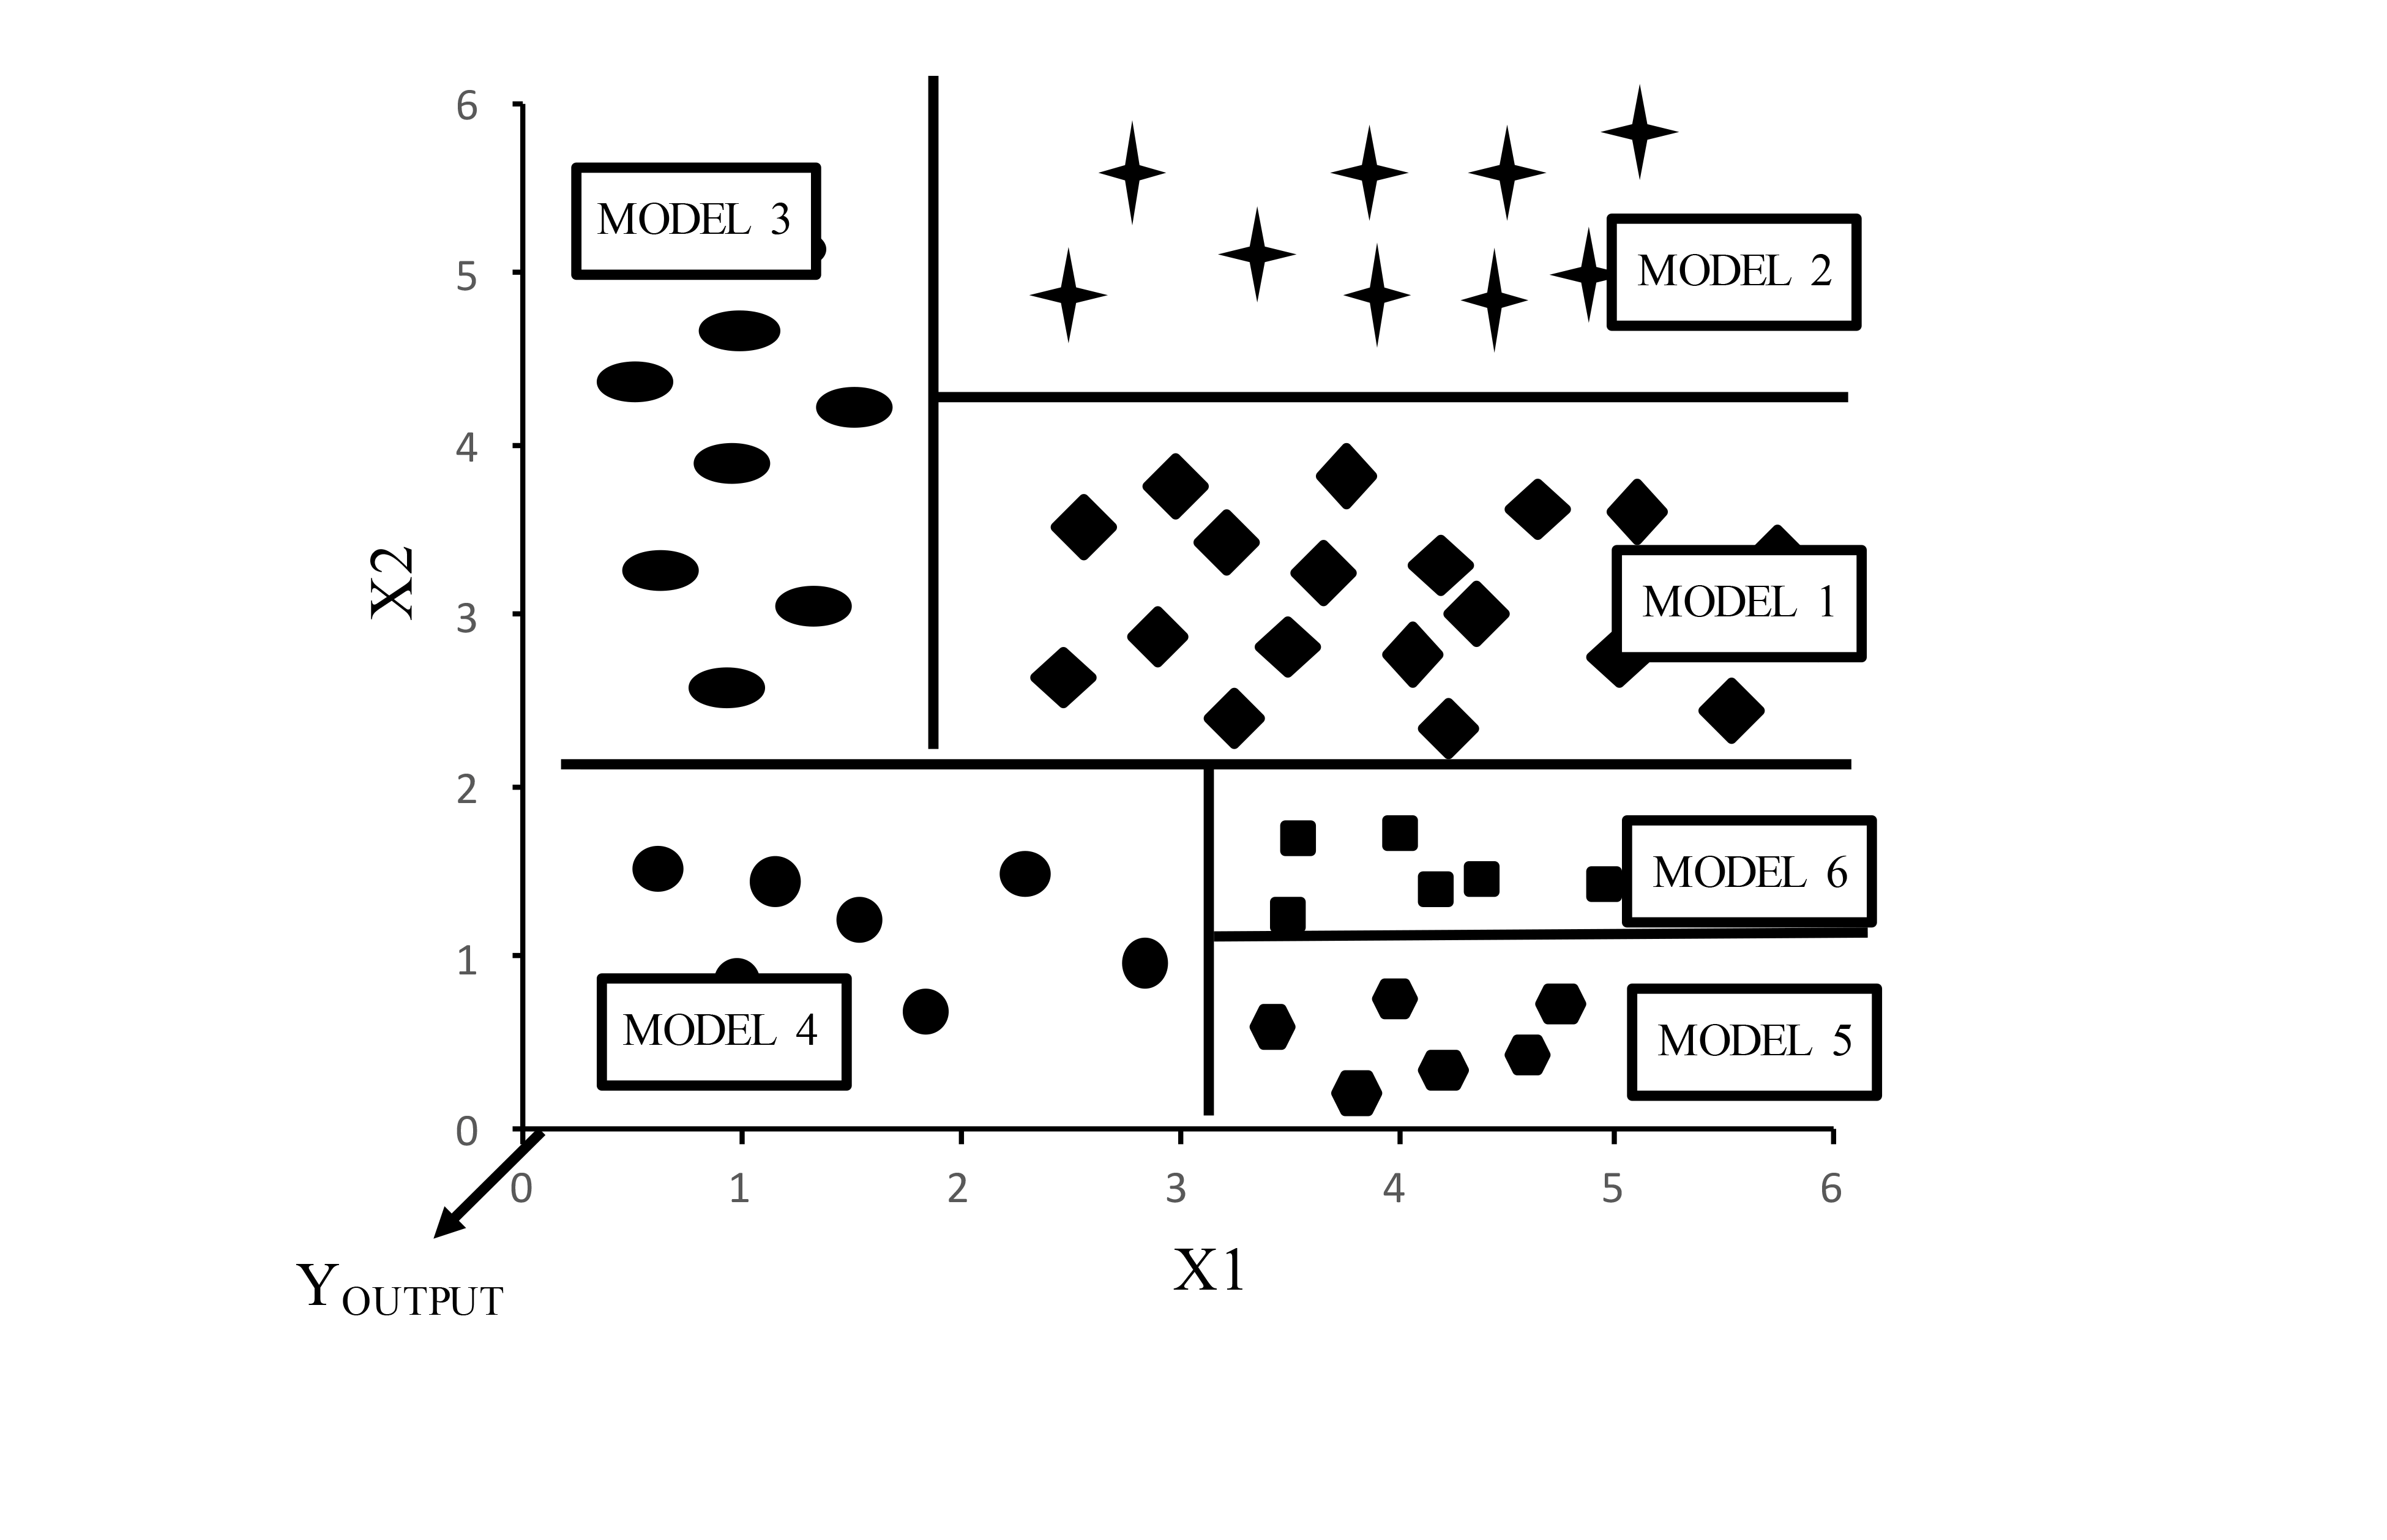
\includegraphics[height=7cm]{splits.png}
\caption{Splitting of the input space (X1 x X2) by M5' model tree algorithm}
\label{fig5}
\end{figure}

\section{Adding another section}
You can show a lot of figures together like these Figures \ref{fig61}, \ref{fig62}, \ref{fig63} below.
\begin{figure} [!htbp]
\centering    
\subfigure[Caption1]{\label{fig61}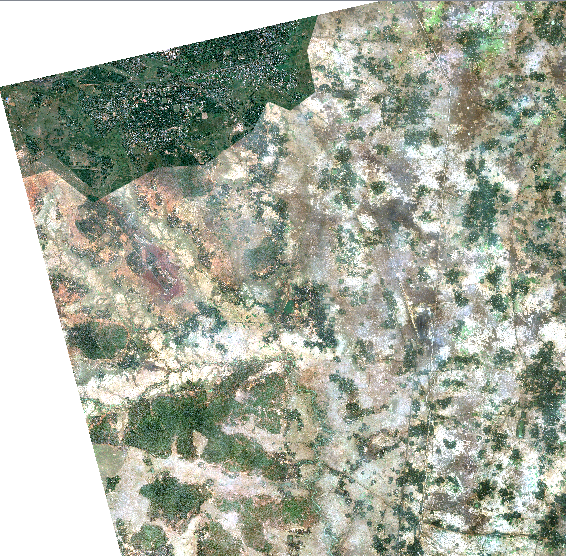
\includegraphics[width=42mm]{data1.png}}
\subfigure[Caption2]{\label{fig62}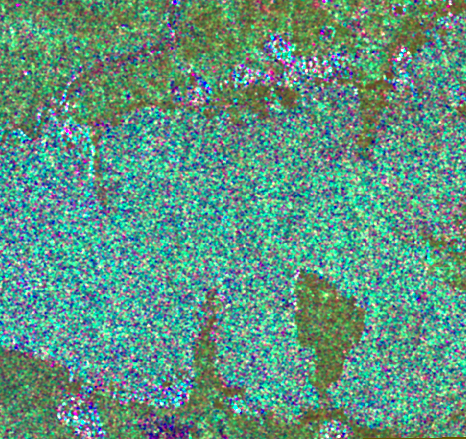
\includegraphics[width=42mm]{data2.png}}
\subfigure[Caption3]{\label{fig63}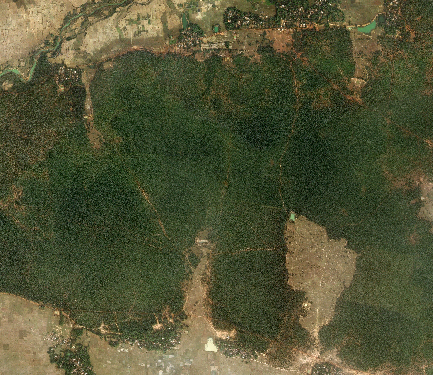
\includegraphics[width=42mm]{data3.png}}
\caption{Figures sample}
\end{figure}
You can add lists into the text like this. 
\begin{itemize}
\settowidth{\leftmargin}{{\Large$\square$}}\advance\leftmargin\labelsep
\itemsep3pt\relax
\renewcommand\labelitemi{{\lower1pt\hbox{\small$\square$}}}
\item	Some sample text item 1. 
\item You may refer to tables \ref{tab1} 
\item Or figures \ref{fig61}
\end{itemize}

Tables can be added like this
\begin{table}[!htbp]
\centering
\caption{Sample table}
\label{tab1}
\begin{tabular}{llll}

\hline
Column 1 & Column 2 & Column 3       \\\hline
1         & Data1 & 13.41179 & 0.9492839 \\
2            & Data2 & 13.39824 & 0.9492952\\\hline
\end{tabular}
\end{table}



% Chapter Template

\chapter{Background Knowledge and Related Works} % Main chapter title

\label{Chapter2} % Change X to a consecutive number; for referencing this chapter elsewhere, use \ref{ChapterX}

\lhead{Chapter 2. \emph{Background Knowledge and Related Works}} % Change X to a consecutive number; this is for the header on each page - perhaps a shortened title
%----------------------------------------------------------------------------------------
%	SECTION 1
%----------------------------------------------------------------------------------------

\section{Stokes Paramters}

In many SAR architectures, the prime objective is to maximize
the measurement potential of a space-based synthetic aperture radar in response to back-scatter from a random field whose elements have unknown orientation relative to the polarity of the radar’s illumination. Measurement potential is maximized if and only if the  data products are the four Stokes parameters of the back-scattered field (or their logical equivalent)\cite{raney2006dual}.

The output from SAR which is recorded is effectively an electromagnetic field nad can be represented  by  the ellipse swept out by its electric potential vector \textit{\textbf{E}}. Stokes proved  that  such  a  field  could  be  represented  by  four real numbers, known as the Stokes parameters $(S_1,S_2,S_3,S_4)$. The  resulting  set  of four  real  numbers,  evaluated  at  each  pixel  location  in  the multilook  image  domain,  comprises  the  fundamental  output data from a SAR \cite{raney2007hybrid}.

In  general,  the  Stokes  parameters and their derived norms provide a set of tools for quantitative image classification.
%----------------------------------------------------------------------------------------
%	SECTION 2
%----------------------------------------------------------------------------------------

\section{m-$\delta$ decomposition}

Another feature that can be derived from Stokes parameters measured in the back-scattered field is the degree of polarization \textit{\textbf{m}}.

\begin{equation}
\label{eq1}
  m = ( S_2^2 + S_3^2 + S_4^2 )^\frac{1}{2}/S_1.
\end{equation}

Another parameter of interest is the relative phase between the two linear \textit{E}-vectors of the back-scattered field.
\begin{equation}
\label{eq2}
  \delta = atan( S_4 / S_3 ) 
\end{equation}
where $-180 < \delta \leq 180$ and the + or - sign of the phase indicates the rotation direction of the polarized field\cite{raney2007hybrid}. m-$\delta$ decomposition is a widely used hybrid polarimetric decomposition technique for land-use classification \cite{chirakkal2017evaluation}.

\section{One-class SVM}
Support vector machines (SVMs) are supervised learning models that analyze data and recognize patterns, and that can be used for both classification and regression tasks. Typically, the SVM algorithm is given a set of training examples labeled as belonging to one of two classes. An SVM model is based on dividing the training sample points into separate categories by as wide a gap as possible, while penalizing training samples that fall on the wrong side of the gap. The SVM model then makes predictions by assigning points to one side of the gap or the other.

Sometimes oversampling is used to replicate the existing samples so that you can create a two-class model, but it is impossible to predict all the new patterns of fraud or system faults from limited examples. Moreover, collection of even limited examples can be expensive \cite{tax2004support}.

Therefore, in one-class SVM, the support vector model is trained on data that has only one class, which is the “normal” class. It infers the properties of normal cases and from these properties can predict which examples are unlike the normal examples \cite{scholkopf2000support}. This is useful for anomaly detection because the scarcity of training examples is what defines anomalies: that is, typically there are very few examples of the network intrusion, fraud, or other anomalous behavior.

 Unlike the Binary SVM method, which tries to find an optimal hyper plane for separating two classes, the One-class SVM classifier constructs an hyper sphere that encloses regions of data distribution \cite{guerbai2014effective}. Hence, the trained One-class SVM classifier contains the maximum of samples in the minimum sphere or enclosed sphere. When a sample is outside of the hyper sphere, it is considered as outlier.

\begin{figure}[]
\centering
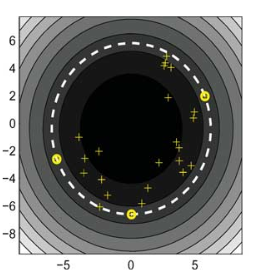
\includegraphics[width=42mm]{data5.png}
\caption{Data description trained on a banana shaped data set.}
\label{fig1}
\end{figure}

To get an intuition on how the one-class SVM works, assume we have a small 2 dimensional banana-shaped data set. we define a model which gives a closed boundary around the data: an hypersphere \cite{tax2004support}. The sphere is characterized by center \textbf{a} and radius \textbf{R} $>$ 0. We minimize the volume of the sphere by minimizing \textbf{$R^2$}, and demand that the sphere contains all training objects. In Figure \ref{fig1} support vectors are indicated by the solid circles, the dashed line is the description boundary.


%----------------------------------------------------------------------------------------
%	SECTION 3
%----------------------------------------------------------------------------------------

\section{Maximum-likelihood classifier}

The maximum likelihood classifier is one of the most popular methods of classification in remote sensing, in which a pixel with the maximum likelihood is classified into the corresponding class \cite{RSGS:2012}. Maximum Likelihood Classifier takes the variance and covariance into account.It does this by computing the distance from the pixel to each class mean value, in units of the standard deviation in that direction, and allocating the pixel to that class with the smallest value in these units of Mahalonobis distance. Mahalonobis distances vary from class to class, and indeed from direction to direction within each class.


%----------------------------------------------------------------------------------------
%	SECTION 4
%----------------------------------------------------------------------------------------

\section{Land Cover Classification using SAR}

Land cover classification is one of the most important applications in the field of polarimetric SAR research. The classification results can be either directly used in mapping and national land resource statistical research, or as the input for other applications. In the fully polarimetric SAR data, the targets’ structure information can be interpreted as the sum of surface scattering, double-bounce scattering and volume scattering. Surface scattering corresponds to rough surfaces such as bare soil and sand land. Double-bounce scattering relates to dihedral corners such as artificial targets’ ground-wall corners. Volume scattering is associated with random oriented dipoles such as the crown of a tree \cite{fang2018land}. As such, polarimetric SAR has the potential to differentiate vegetation, bare land, buildings, water bodies, and so on.

One of the most extensively used features for classification are Entropy \textbf{H},  Anisotropy \textbf{A} and scattering angle $\alpha$ \cite{lee2009polarimetric}. The complex wishart classifier described in \cite{lee2009polarimetric} takes into consideration various properties of the backscatter field. Ocean surface and flat ground typically have the characteristics of Bragg scattering (odd bounce),city
blocks, buildings, and hard targets have the characteristics of double bounce scattering (even bounce) and forest, heavy vegetation have the characteristics of volume scattering(diffuse scattering). Consequently, this classification algorithm provides information for terrain type identification. The medium’s scattering mechanisms, characterized by entropy \textit{B} and scattering angle $\alpha$, are used for classification.

%----------------------------------------------------------------------------------------
%	SECTION 5
%----------------------------------------------------------------------------------------

\section{Tools Used}

Various tools were used in order to process the SAR data, extract the features needed to classify, process the ground-truth by labelling reference pixels. All the code that was created for the project was written in python language. 
%-----------------------------------
%	SUBSECTION 1
%-----------------------------------
\subsection{PolSARpro}

PolSARpro is a project that works to provide a tool for self-education in the field of polarimetric SAR data analysis and a comprehensive suite of functions for the scientific exploitation of fully and partially polarimetric data and the development of applications for such data.

The PolSARpro software is controlled through a user-friendly, intuitive graphical interface, which enables the user to select a function, set its parameters and then run it. The software environment is flexible, developed to be accessible to a wide range of users - from novices to experts - in the field of Polarimetric SAR data processing.PolSARpro data processing routines are written in C (greater than 1000 routines) and the GUI is written in Tcl-Tk. The software is accompanied by in-depth online help, technical documentation for developers and a tutorial programme permitting self-education to a high level\cite{pottier2009overview}.

%-----------------------------------
%	SUBSECTION 2
%-----------------------------------

\subsection{QGIS}
QGIS is a popular open-source geographic information system (GIS) with advanced capabilities\cite{qgis2015qgis}. QGIS functions as GIS software, allowing users to analyze and edit spatial information, in addition to composing and exporting graphical maps. QGIS supports both raster and vector layers; vector data is stored as either point, line, or polygon features. Multiple formats of raster images are supported, and the software can geo-reference images.

\subsection{LIBSVM}
LIBSVM is an integrated software for support vector classification.It supports multi-class classification \cite{chang2011libsvm}. LIBSVM is a popular open source machine learning library, developed at the National Taiwan University and written in C++ though with a C API. LIBSVM implements the SMO algorithm for kernelized support vector machines (SVMs), supporting classification and regression.We used the python interface of LIBSVM for our One Class SVM.

%----------------------------------------------------------------------------------------
%	SECTION 2
%----------------------------------------------------------------------------------------
 
% Chapter Template

\chapter{Methodology} % Main chapter title

\label{Chapter4} % Change X to a consecutive number; for referencing this chapter elsewhere, use \ref{ChapterX}

\lhead{Chapter 4. \emph{Methodology}} % Change X to a consecutive number; this is for the header on each page - perhaps a shortened title

%----------------------------------------------------------------------------------------
%	SECTION 1
%----------------------------------------------------------------------------------------

\section{Study Area and Data Processing}

For this study, the test site chosen was Kharagpur, Salua its surrounding region in West Bengal, India. The site covers predominantly agricultural fields and forest cover along with some urban buildup. RISAT-1 data has been acquired on January 4, 2013 with a central latitude of 22.208289$\degree$N,central longitude of 87.414885$\degree$E and at incidence angle of 48.11354$\degree$. Using polSARpro and QGIS software this single look complex data was used to produce a geo-referenced primitive RGB output corresponding to the complex data and the four geo-referenced stokes parameter TIFF files. These four images were used to derive the features used to classify the area under study.
\begin{figure}[!htbp]
\centering
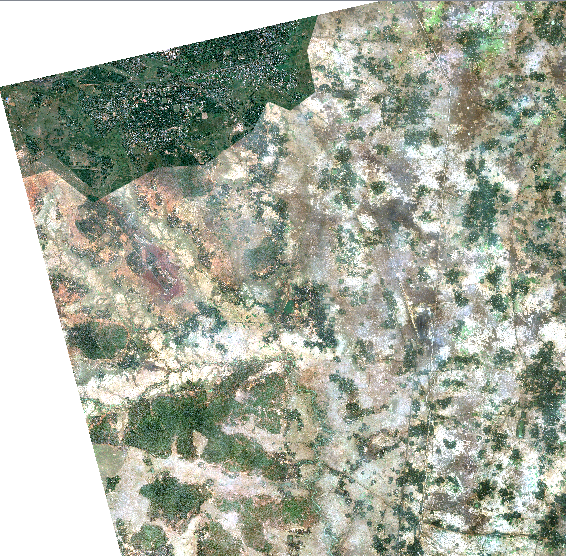
\includegraphics[width=50mm]{data1.png}
\caption{Google Earth image of the area under study. }
\label{fig2}
\end{figure}

Groundtruth for one-class SVM only contained reference pixels of forest cover in the whole area of study. Groundtruth was acquired from the past decade's topology charts from the Government of India. Total number of pixels in the image is 49,006,994. Total number of labelled pixels is 4,915,924, which is approximately 10$\%$ of the total pixels under study.

Groundtruth for maximum likelihood classifier required negative instances of forest cover, this was added manually by going through the Google Earth image and the RGB output image, which showed patterns, labelling agricultural, water bodies and urban buildup as the second class other than forest. We select the region of interest for the non-forest class using QGIS plugin tool. Number of pixels in this class was also fixed to be same as forest pixels.

\begin{figure}[!htbp]
\centering
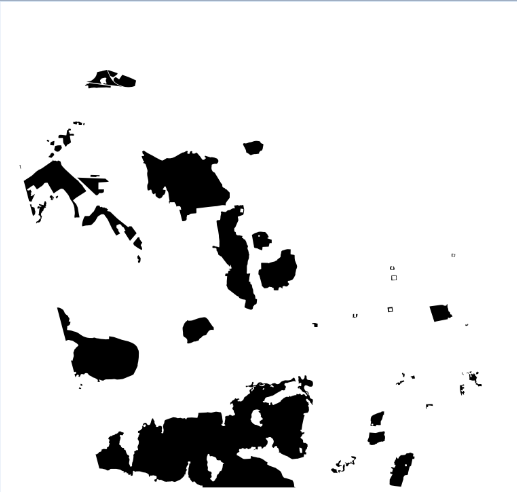
\includegraphics[width=60mm]{Pictures/data6.png}
\caption{Groundtruth showing black pixels as forest. }
\label{fig3}
\end{figure}

In case of maximum likelihood classifier, we require the groundtruth to be saved as spectral signature files, this is done using the QGIS software plugin tool. m-$\delta$ decompostion is done on the stokes parmaters images using the equations mentioned \ref{eq1} and \ref{eq2} we used our own python code to produce another image.  

\begin{figure}[!htbp]
\centering
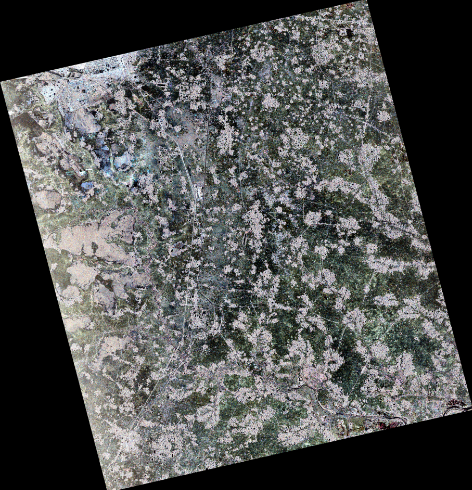
\includegraphics[width=60mm]{Pictures/data7.png}
\caption{RGB output image from polSARpro. }
\label{fig4}
\end{figure}


%----------------------------------------------------------------------------------------
%	SECTION 2
%----------------------------------------------------------------------------------------

\section{Image Classification}
We are trying to detect forest area in the dataset using two machine learning classification models, namely maximum likelihood classification and one class SVM. We will try to detect forest using two types of features, first the stokes parameter, secondly m-$\delta$ values. 

\subsection{Maximum Likelihood Classifier}

The classifier considers both the variances and covariances of the class signatures when assigning each cell to one of the classes represented in the signature file. A class can be characterized by the mean vector and the covariance matrix. Given these two characteristics for each pixel value, the statistical probability is computed for each class to determine the membership of the pixels to the class. Each pixel is assigned to the class to which it has the highest probability of being a member.

 The classifier we used in our work uses QGIS Semi-Automatic Classification Plugin Tool \cite{congedo2016semi}. When a maximum likelihood classification is performed, first the mean vector and covariance matrix is computed from the signature files given as groundtruth. Then the statistical probabilty is computed for each pixel in the whole image. We do this for both stokes paramters and m-$\delta$ value. In case of stokes paramter we add all four separate stokes parameter images as input to calculate the mean vector and covariance matrix. 
 
 We finally generate a TIFF file that is georeferenced to the location of the dataset and can then compare the results visually too in QGIS.


\subsection{One Class SVM}

We used the python interface for LIBSVM to implement the One Class SVM. The procedure that we followed :
\begin{itemize}
\item Transform the data to the format of the SVM package. 	 
\item Use cross-validation to find the best parameter  $\nu$ and $\gamma$.
\item Use the best parameter $\nu$ and $\gamma$ to train the whole training set.
\item Test on the whole dataset.
\end{itemize}
Before we train and test we have to decide on the size of the split of the complete ground truth; this needs to be done for various sizes to compare the accuracy.

\subsubsection{Training}\label{train}

We only have positive instances of the forest cover, inorder to train this we have to first create two vectors \textbf{X} (features or attributes) and \textbf{Y} (label). Each pixel in the training set has a value of +1 in \textbf{Y} and all four corresponding stokes parameter pixels(four dimensional) in \textbf{X} for classification with stokes parameters as feature, this changes to corresponding m-$\delta$ pixels (two dimensional) when we are classifying on the m-$\delta$ features. 

We then construct a problem in python format, This done using the svm\_problem() function predefined in the svmutil package. The parameters are set using the svm\_parameter() function, here we have to specify that our problem is a one-class SVM problem, uses an RBF kernel and set the value for the two parameters defined for the 
One class SVM namely $\nu$ (nu) and $\gamma$(gamma). After the problem is defined and the parameters are set, we can train and save the model for future use. Training typically takes 48 hours and we can save this time by saving the model when using the  same parameters and training set. 

\subsubsection{Testing}

In addition to testing on the test set we defined, we also have to test the data on the whole dataset to detect forest cover in unknown regions. Therefore, we have to have the whole dataset prepared in the same format discussed in \ref{train} as \textbf{Y} and \textbf{X}, for unknown pixels we denote values in \textbf{Y} as -1.
We use the svm\_predict() function to predict the label of the unknown pixel as either 1(for forest) or -1(for non-forest). After predicting for the entire dataset we create a final output image that can be viewed to assess the accuracy.

\subsubsection{Hyper-parameter tuning}

This is an important step in the classification using one class SVM. There are two parameters for an RBF kernel: $\nu$ and $\gamma$. It is not known beforehand
which $\nu$ and $\gamma$ are best for the given problem; consequently some kind of model selection (parameter search) must be done. The goal is to identify good ($\nu$ , $\gamma$) so that the classifier can accurately predict unknown data (i.e. testing data).

We try to find the best parameter pair using two techniques: grid-search and cross-validation.In n-fold cross-validation, we first divide the training set into n subsets of equal size. Sequentially one subset is tested using the classifier trained on the remaining n − 1 subsets. Thus, each instance of the whole training set is predicted once so the cross-validation accuracy is the percentage of data which are correctly classified \cite{hsu2003practical}.

Grid-search on $\nu$ and $\gamma$ using cross-validation is the recommended approach as in \cite{hsu2003practical}. Various pairs of ($\nu$ , $\gamma$) values are tried and the one with the best cross-validation accuracy is
picked. 



 
% Chapter Template

\chapter{Result} % Main chapter title

\label{Chapter4} % Change X to a consecutive number; for referencing this chapter elsewhere, use \ref{ChapterX}

\lhead{Chapter 4. \emph{Result}} % Change X to a consecutive number; this is for the header on each page - perhaps a shortened title

%----------------------------------------------------------------------------------------
%	SECTION 1
%----------------------------------------------------------------------------------------

\section{Maximum likelihood Classifier}

Implemented and executed Maximum Likelihood Classifier for stokes parameter with an overall accuracy = 79\%. 

\begin{table}[!htbp]
\centering
\caption{Confusion Matrix for ML Classifier}
\label{tab1}
\begin{tabular}{llll}

\hline
Class  & Forest & Non-Forest & Total Classified pixels      \\\hline
Forest         & 4,129,376 & 1,179,822 & 5,309,198 \\\hline
Non-Forest            & 786,548 & 3,736,102 & 4,522,650 \\\hline
Total ground truth pixels   & 4,915,924 & 4,915,924 & 9,831,848
\end{tabular}
\end{table}

Producer Accuracy for forest class = 83.9\%

Producer Accuracy for non-forest class = 75.9\%

User Accuracy for forest class = 77.7\%

User Accuracy for non-forest class = 82.6\%


%-----------------------------------
%	SUBSECTION 1
%-----------------------------------
\subsection{Discussion}
Upon Visually analyzing the whole image, we can observe that a huge number of pixels that were urban buildup which was not included in the groundtruth.  Figures \ref{fig61}, \ref{fig62}, \ref{fig63} below show a cropped portion of the whole image where forest area can be seen clearly.
\begin{figure} [!htbp]
\centering    
\subfigure[google earth image]{\label{fig61}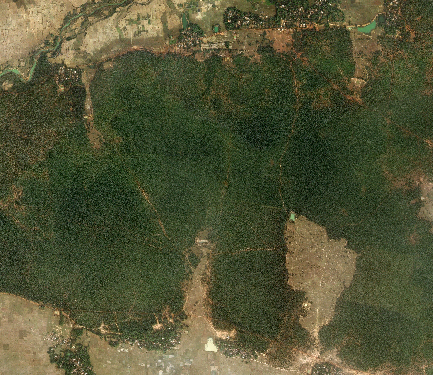
\includegraphics[width=40mm]{data3.png}}
\subfigure[RGB colour composite]{\label{fig62}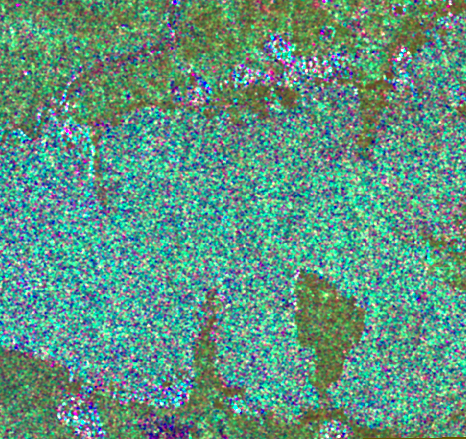
\includegraphics[width=40mm]{data2.png}}
\subfigure[classified image]{\label{fig63}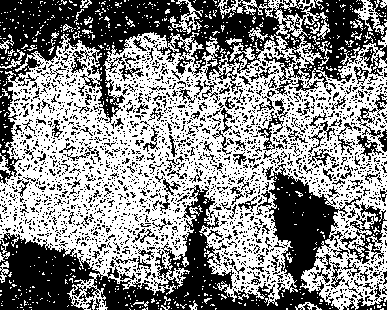
\includegraphics[width=40mm]{data4.png}}
\caption{Figures sample}
\end{figure}
The classifier required additional negative instances as ground truth to actually run and hence introduced difficulty in labelling the same. Maximum Likelihood Classifier used in the QGIS plugin tool assumes that the data pixels are normally distributed, but our data follows a complex distribution other than gaussian and hence did not give a very high accuracy . 
\begin{figure} [!htbp]
\centering    
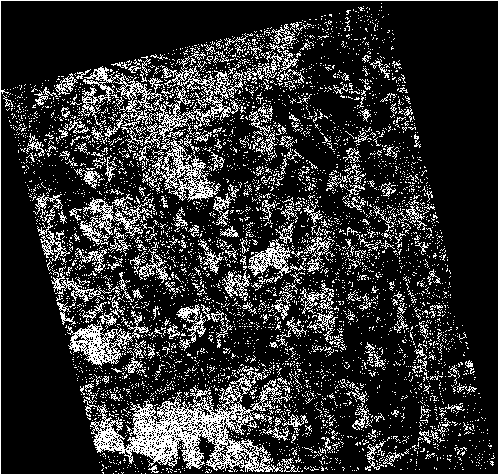
\includegraphics[width=50mm]{data8.png}
\caption{Final output image}
\end{figure}

%----------------------------------------------------------------------------------------
%	SECTION 2
%----------------------------------------------------------------------------------------

\section{One class SVM}

10-fold cross validation was done along with grid search to get the $\nu$ and $\gamma$ parameters and a producer accuracy of 99.08$\%$. for the stokes parameters feature and an accuracy of 98.81$\%$ for m-$\delta$ as feature used for classification.

\begin{table}[!htbp]
\centering
\caption{Parameter values}
\label{tab2}
\begin{tabular}{llll}

\hline
Feature  & $\nu$ & $\gamma$     \\\hline
Stokes parameters   & $9 \times 10^{-4}.$ & $3 \times 10^{-6}.$ \\\hline
m-$\delta$            & $9 \times 10^{-4}.$ & $1 \times 10^{-6}.$ \\\hline
\end{tabular}
\end{table}

%-----------------------------------
%	SUBSECTION 2
%-----------------------------------

\subsection{Discussion}
Even though, we got a good producer accuracy on the given groundtruth, when the classifier was used to predict the whole dataset, visually it was found that a large number of pixels were mispredicted as forest. 
 
% Chapter Template

\chapter{Conclusion } % Main chapter title

\label{Chapter5} % Change X to a consecutive number; for referencing this chapter elsewhere, use \ref{ChapterX}

\lhead{Chapter 5. \emph{Conclusion}} % Change X to a consecutive number; this is for the header on each page - perhaps a shortened title

%----------------------------------------------------------------------------------------
%	SECTION 1
%----------------------------------------------------------------------------------------

The utilization of features such as Stokes parameter were helpful in detecting forest area in the given dataset. Comparatively, classification with m-$\delta$ values as the feature showed lesser accuracy than when classification is done with stokes parameter as the feature. Maximum Likelihood Classifier requires atleast two classes to work and hence required us to manually label non-forest area, One Class SVM doesn't require negative instances and can hence remove this difficulty. 
% Chapter Template

\chapter{Future Work} % Main chapter title

\label{Chapter6} % Change X to a consecutive number; for referencing this chapter elsewhere, use \ref{ChapterX}

\lhead{Chapter 6. \emph{Future Work}} % Change X to a consecutive number; this is for the header on each page - perhaps a shortened title

%----------------------------------------------------------------------------------------
%	SECTION 1
%----------------------------------------------------------------------------------------

One class SVM when predicting on the whole dataset visually mispredicted a lot of pixels, this might be due to choosing non-optimal parameters or due to not scaling the data attributes. More optimal parameters can be found. Scaling can improve the accuracy significantly if properly done. Possibility of developing unsupervised classification algorithms based on stokes parameter can be investigated in the future. Image classification methods using Deep Neural Networks in SAR data have surfaced and can be investigated in the future.  
%\input{Chapters/Chapter7} 
%\input{Chapters/Chapter7} 

%----------------------------------------------------------------------------------------
%	THESIS CONTENT - APPENDICES
%----------------------------------------------------------------------------------------

\addtocontents{toc}{\vspace{2em}} % Add a gap in the Contents, for aesthetics


\addtocontents{toc}{} % Add a gap in the Contents, for aesthetics

\backmatter

%----------------------------------------------------------------------------------------
%	BIBLIOGRAPHY
%----------------------------------------------------------------------------------------
%\nocite{*}
\label{Bibliography}

\lhead{\emph{Bibliography}} % Change the page header to say "Bibliography"

\bibliographystyle{apalike} % Use the "custom" BibTeX style for formatting the Bibliography

\bibliography{Bibliography} % The references (bibliography) information are stored in the file named "Bibliography.bib"

\end{document}  
